%%%%%%%%%%%%%%%%%%%%%%%%%%%%%%%%%%%%%%%%%%%%%%%%%%%%%%%%%%%%%%%%
%%                                                            %%
%%   essentialsOfLatin, Italian translation 2017              %%
%%                                                            %%
%% From:  Henry C. Pearson, Essentials Of Latin For Beginners %%
%%        (1915, New York, American Book Company)             %%
%%                                                            %%
%%    https://archive.org/details/essentialslatin04peargoog   %%
%%                                                            %%
%% Translated by g.p.ciceri <gp.ciceri@gmail.com>             %%
%% ---------------------------------------------------------- %%
%% This translation is Licensed under                         %%
%% Creative Commons Attribution-ShareAlike 4.0 International  %%
%% https://creativecommons.org/licenses/by-sa/4.0/            %%
%%                                                            %%
%%%%%%%%%%%%%%%%%%%%%%%%%%%%%%%%%%%%%%%%%%%%%%%%%%%%%%%%%%%%%%%%

% āēīōū
% ăĕĭŏŭ




\documentclass[nols]{tufte-handout}

%\geometry{showframe} % display margins for debugging page layout

\usepackage{fontspec}
\usepackage{ifxetex}
\setmainfont[Path=./fonts/palatino-linotype/, ItalicFont=palai.ttf, BoldFont=palab.ttf]{pala.ttf}


% \defaultfontfeatures{Mapping=tex-text}
% \setromanfont[Path=./fonts/TeX-Gyre-Schola/,Mapping=tex-text]{TeX Gyre Schola}
% \setsansfont[Path=./fonts/TeX-Gyre-Heros/,Scale=MatchLowercase,Mapping=tex-text]{TeX Gyre Heros}
% \setmonofont[Path=./fonts/TeX-Gyre-Cursor/,Scale=MatchLowercase]{TeX Gyre Cursor}

\usepackage{lipsum}
\usepackage{url}
\usepackage{longtable}
\usepackage{stackengine}

\usepackage{graphicx} % allow embedded images
  \setkeys{Gin}{width=\linewidth,totalheight=\textheight,keepaspectratio}
  \graphicspath{{graphics/}} % set of paths to search for images
\usepackage{amsmath}  % extended mathematics
\usepackage{booktabs} % book-quality tables
\usepackage{units}    % non-stacked fractions and better unit spacing
\usepackage{multicol} % multiple column layout facilities
\usepackage{lipsum}   % filler text
\usepackage{fancyvrb} % extended verbatim environments
  \fvset{fontsize=\normalsize}% default font size for fancy-verbatim environments

% Standardize command font styles and environments
\newcommand{\doccmd}[1]{\texttt{\textbackslash#1}}% command name -- adds backslash automatically
\newcommand{\docopt}[1]{\ensuremath{\langle}\textrm{\textit{#1}}\ensuremath{\rangle}}% optional command argument
\newcommand{\docarg}[1]{\textrm{\textit{#1}}}% (required) command argument
\newcommand{\docenv}[1]{\textsf{#1}}% environment name
\newcommand{\docpkg}[1]{\texttt{#1}}% package name
\newcommand{\doccls}[1]{\texttt{#1}}% document class name
\newcommand{\docclsopt}[1]{\texttt{#1}}% document class option name
\newenvironment{docspec}{\begin{quote}\noindent}{\end{quote}}% command specification environment

% concetti morfosintattici
\usepackage{xspace} 
\newcommand{\noun}{\textsc{sostantivo}\xspace}
\newcommand{\nouns}{\textsc{sostantivi}\xspace}
\newcommand{\adject}{\textsc{aggettivo}\xspace}
\newcommand{\adjects}{\textsc{aggettivi}\xspace}
\newcommand{\gnumber}{\textsc{numero}\xspace}
\newcommand{\gnumbers}{\textsc{numeri}\xspace}
\newcommand{\gender}{\textsc{genere}\xspace}
\newcommand{\genders}{\textsc{generi}\xspace}
\newcommand{\gcase}{\textsc{caso}\xspace}
\newcommand{\gcases}{\textsc{casi}\xspace}
\newcommand{\tense}{\textsc{tempo}\xspace}
\newcommand{\mood}{\textsc{modo}\xspace}
\newcommand{\gverb}{\textsc{verbo}\xspace}
\newcommand{\gverbs}{\textsc{verbi}\xspace}
\newcommand{\adjective}{\textsc{aggettivo}\xspace}
\newcommand{\nom}{\textsc{nom}\xspace}
\newcommand{\gen}{\textsc{gen}\xspace}
\newcommand{\dat}{\textsc{dat}\xspace}
\newcommand{\acc}{\textsc{acc}\xspace}
\newcommand{\voc}{\textsc{voc}\xspace}
\newcommand{\abl}{\textsc{abl}\xspace}
\newcommand{\gexit}{\textsc{uscita}\xspace}
\newcommand{\gexits}{\textsc{uscite}\xspace}
\newcommand{\declinazione}{\textsc{declinazione}\xspace}
\newcommand{\masc}{\textsc{maschile}\xspace}
\newcommand{\femm}{\textsc{femminile}\xspace}
\newcommand{\neut}{\textsc{neutro}\xspace}

\newcommand{\indic}{\textsc{indicativo}\xspace}
\newcommand{\imper}{\textsc{imperativo}\xspace}
\newcommand{\gcong}{\textsc{congiuntivo}\xspace}
\newcommand{\ott}{\textsc{ottativo}\xspace}
\newcommand{\partic}{\textsc{participio}\xspace}
\newcommand{\infin}{\textsc{infinito}\xspace}

\newcommand{\pres}{\textsc{presente}\xspace}
\newcommand{\imperf}{\textsc{imperfetto}\xspace}
\newcommand{\aor}{\textsc{aoristo}\xspace}
\newcommand{\fut}{\textsc{futuro}\xspace}
\newcommand{\perf}{\textsc{perfetto}\xspace}
\newcommand{\pperf}{\textsc{piuccheperfetto}\xspace}

\newcommand{\sing}{\textsc{singolare}\xspace}
\newcommand{\plur}{\textsc{plurale}\xspace}
\newcommand{\dual}{\textsc{duale}\xspace}

\newcommand{\si}{\textsc{sing}\xspace}
\newcommand{\pl}{\textsc{plur}\xspace}
\newcommand{\du}{\textsc{dual}\xspace}

\newcommand{\att}{\textsc{attivo}\xspace}
\newcommand{\med}{\textsc{medio}\xspace}
\newcommand{\pass}{\textsc{passivo}\xspace}
\newcommand{\medpass}{\textsc{medio-passivo}\xspace}


% italianitudini
\renewcommand{\figurename}{Figura}
\renewcommand{\tablename}{Tabella}
\renewcommand{\contentsname}{Indice}

% fix per un qualche problema
\ifxetex
  \newcommand{\textls}[2][5]{%
    \begingroup\addfontfeatures{LetterSpace=#1}#2\endgroup
  }
  \renewcommand{\allcapsspacing}[1]{\textls[15]{#1}}
  \renewcommand{\smallcapsspacing}[1]{\textls[10]{#1}}
  \renewcommand{\allcaps}[1]{\textls[15]{\MakeTextUppercase{#1}}}
  \renewcommand{\smallcaps}[1]{\smallcapsspacing{\scshape\MakeTextLowercase{#1}}}
  \renewcommand{\textsc}[1]{\smallcapsspacing{\textsmallcaps{#1}}}
\fi

% too many float...
\extrafloats{100}
% āēīōū
% ăĕĭŏŭ

\title{Essentials Of Latin. Elementi di Latino. \newline Lezione XII - Prima coniugazione (continua). Il Perfetto. Ablativo di mezzo.}

\author[gpciceri]{a cura di Milagathòs: Milo's help to enjoy humanities.}

\date{24 Febbrajo 2017} % without \date command, current date is supplied


\begin{document}

\hyphenation{co-niu-ga-zio-ne}

\maketitle% this prints the handout title, author, and date

\begin{marginfigure}[-2.5cm]
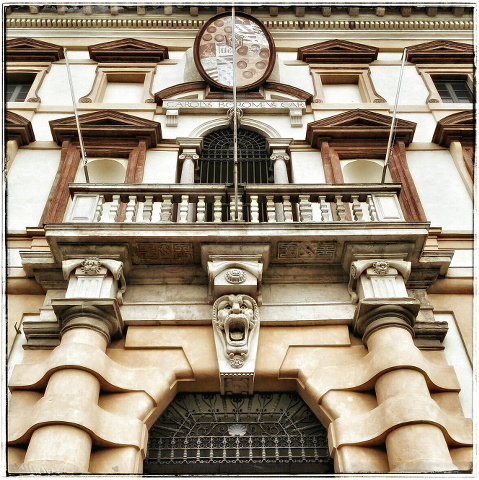
\includegraphics{smallthumb-lesson_I.jpeg}
\setfloatalignment{b}
\end{marginfigure}


\begin{abstract}
\noindent
Queste lezioni riprendono il testo introduttivo al Latino di Pearson\cite{pearson1915}, del quale seguono la numerazione; la struttura di ogni lezione è piuttosto regolare: inizia con \textsc{cenni di morfologia e di sintassi latina}, seguita da un \textsc{piccolo vocabolario} per il lessico; ci sono infine vari \textsc{esercizi} di traduzione e di composizione latina.

\bigskip
\noindent
Lezione XII - Prima coniugazione (continua). Il Perfetto. Ablativo di mezzo. Vocabolario, esercizi.
\end{abstract}

%\printclassoptions

% āēīōū
% ăĕĭŏŭ

\newthought{92. Prima Coniugazione, Perfetto.} 

\begin{fullwidth}
\begin{table}[!htbp]
  \centering
  \begin{tabular}{l l l l}
    %\toprule
	
	\multicolumn{4}{c}{\textsc{Indicativo Perfetto Attivo} di \textbf{amō}, \textit{io amo}} \\
	
	& \multicolumn{1}{c}{\textsc{Singolare}} & \hspace{10mm} & \multicolumn{1}{c}{\textsc{Uscite}} \\

    \textsc{1.} & amāv\textbf{ī}, \textit{io amai, ho amato, ebbi amato}   & \hspace{10mm} & \textbf{-ī}   \\
    \textsc{2.} & amāv\textbf{istī}, \textit{tu amasti, ecc.}   & \hspace{10mm} & \textbf{-istī}  \\
    \textsc{3.} & amāv\textbf{it}, \textit{egli amò, ecc.} & \hspace{10mm} & \textbf{-it}   \\
   
	& \multicolumn{1}{c}{\textsc{Plurale}} & \hspace{20mm} &  \\
	
    \textsc{1.} & amāv\textbf{imus}, \textit{noi amammo, ecc.}   & \hspace{10mm} & \textbf{-imus}   \\
    \textsc{2.} & amāv\textbf{istis}, \textit{voi amaste, ecc.}   & \hspace{10mm} & \textbf{-istis}  \\
    \textsc{3.} & amāv\textbf{ērunt}, \textit{essi amarono, ecc.} & \hspace{10mm} & \textbf{-ērunt}   \\
	
    %\bottomrule
  \end{tabular}
  %\caption[bottom]{Prima Coniugazione, Perfetto.}
  \label{tab:normaltab}
  %\zsavepos{pos:normaltab}
\end{table}
\end{fullwidth}

\newthought{Osservazioni}
\begin{itemize}
\item[\textsc{1.}] \textit{Le uscite personali del perfetto sono le medesime in tutte le coniugazioni}. 
Queste uscite sono diverse da quelle dei tempi presente, imperfetto, futuro.
\item[\textsc{2.}] Utilizzo del tempo perfetto. Il perfetto indica un'azione o uno stato \textit{completato} (nel passato) al tempo attuale, l'imperfetto un'azione o stato \textit{che prosegue, ripetuta, continuata} nel passato. 
\item[\textsc{3.}] Coniuga il perfetto dei verbi alla sezione (88.).
\end{itemize}

\newthought{93. Frasi Modello.} Esamina le seguenti frasi:
\begin{itemize}
\item[\textsc{1.}] \textbf{Hastis et sagittis pugnabant}, \textit{combattevano con lance e frecce}.  
\item[\textsc{2.}] \textbf{Equis frumentum portabimus}, \textit{porteremo il grano per mezzo di cavalli}.  
\end{itemize}

Osserva che gli ablativi \textbf{hastis, sagittis, equis} esprimono il \textit{mezzo} o lo \textit{strumento}: 
le cose per mezzo delle quali si compie l'azione descritta dal verbo. 

\newthought{94. Regola \textemdash Ablativo di Mezzo o di Strumento.} Il mezzo o lo strumento di un'azione è espresso in ablativo semplice, senza preposizione.

% āēīōū
% ăĕĭŏŭ

\newthought{95. Vocabolario} 

\begin{multicols}{2}
    \noindent \hangindent=1em \textbf{legatus, -ī}, m., \textit{ambasciatore, luogotenente}.  \\
    \noindent \hangindent=1em \textbf{Graecus, -ī}, n., \textit{un greco}.  \\
    \noindent \hangindent=1em \textbf{pauci, ae, a}, agg. pl., \textit{pochi}.  \\
	
	\noindent \hangindent=1em \textbf{superō, -as, -āvī, -ātum, -āre}, v.tr., \textit{supero, conquisto, ho la meglio su}.  \\
	\noindent \hangindent=1em \textbf{armō, -as, -āvī, -ātum, -āre}, v.tr., \textit{armare, equipaggiare}.  \\
	\noindent \hangindent=1em \textbf{dō, das, dedī, dātum, dāre}, v.tr.(perf.irr.), \textit{dare}.  \\
	\noindent \hangindent=1em \textbf{oppugnō, -as, -āvī, -ātum, -āre}, v.tr., \textit{attaccare, assediare}.  \\
	
	\noindent \hangindent=1em \textbf{arma, -ōrum}, n.pl., \textit{armi}.  \\
	\noindent \hangindent=1em \textbf{hiberna, -ōrum}, n.pl., \textit{accampamenti invernali}.  \\
    \noindent \hangindent=1em \textbf{Helvetius, -ī}, n., \textit{un elvezio}.  \\
	
\end{multicols}
% āēīōū
% ăĕĭŏŭ

\newthought{96. Esercizi di Ripasso}
\\
\textsc{I.} \quad
\textsc{1.}~Dominus meus dona filiis dabit. \quad
\textsc{2.}~Nautae fidi contra Romanos pugnabant. \quad
\textsc{3.}~Tela idonea in castra portabunt. \quad
\textsc{4.}~Copia magna telorum est in loco. \quad
\textsc{5.}~Servi pigri multum frumentum in aedificia non portabant. \quad
\textsc{6.}~Locus magno proelio non erit idoneus.
\\
\textsc{II.} \quad
\textsc{1.}~L'accampamento dei romani era grande. \quad
\textsc{2.}~Perché diede armi agli abitanti? \quad
\textsc{3.}~Porteremo molte lance e frecce in città. \quad
\textsc{4.}~Apprezzava le forze (armate) della regina.


\newthought{97. Esercizi}
\\
\textsc{I.} \quad
\textsc{1.}~Pugnavisti; dedistine? laudavimus. \quad
\textsc{2.}~Incolae oppidi multa arma comparaverunt. \quad
\textsc{3.}~Helvetii oppidum saxis et armis oppugnabant. \quad
\textsc{4.}~Equis in aedificium cibum portavit. \quad
\textsc{5.}~Pauca arma viris dedimus. \quad
\textsc{6.}~Cur Romani Graecos superaverunt ? \quad
\textsc{7.}~Servi multum frumentum in hiberna portaverunt. \quad
\textsc{8.}~Romani Helvetiorum oppida sagittis et pilis oppugnabant. \quad
\textsc{9.}~Incolas insulae tells armabimus. \quad
\textsc{10.}~In hibernis sunt pauca tela et multus cibus. \quad
\textsc{11.}~Gallos hastis et sagittis superavit. \quad
\textsc{12.}~Locus hibernis idoneus est. 
\\
\textsc{II.} \quad
\textsc{1.}~Avete dato; incolpò egli? \quad
\textsc{2.}~Abbiamo equipaggiato; conquistavano; diede. \quad
\textsc{3.}~I Galli combatterono con lance e frecce. \quad
\textsc{4.}~I Romani hanno attaccato l'accampamento dei Greci. \quad
\textsc{5.}~Sollevò gli Elvezi per mezzo di ricompense. 

{(444.) Lettura. Un Fidanzamento Burrascoso} 
Roma parvum oppidum erat, ubi Romulus in terris erat. 
Incolae viri erant, sed feminae in oppido non erant. 
Romuli legatl multos agricolas et multas feminas et pulchras puellas in oppidum convocaverunt. 
Telis idoneis, pilis, gladiis, hastis, incolae pugnabant. 
Feminas asperum proelium delectabat. Sed Romuli consilium malum erat. 
Viri validi puellas teneras in aedificia portaverunt. 
Tum \sidenote{\textbf{tum}, \textit{allora}}superbi agricolae armis Romanos oppugnaverunt. 
Sed Romulus et Romuli amici agricolas superabant. 
Tum miserae agricolarum filiae parvos liberos in proelium portaverunt et viros vocaverunt: 
“Semper viros et liberos amabimus. Cur pugnatis? Nonne filias et filiarum liberos amatis?”


\begin{figure}[!b]
  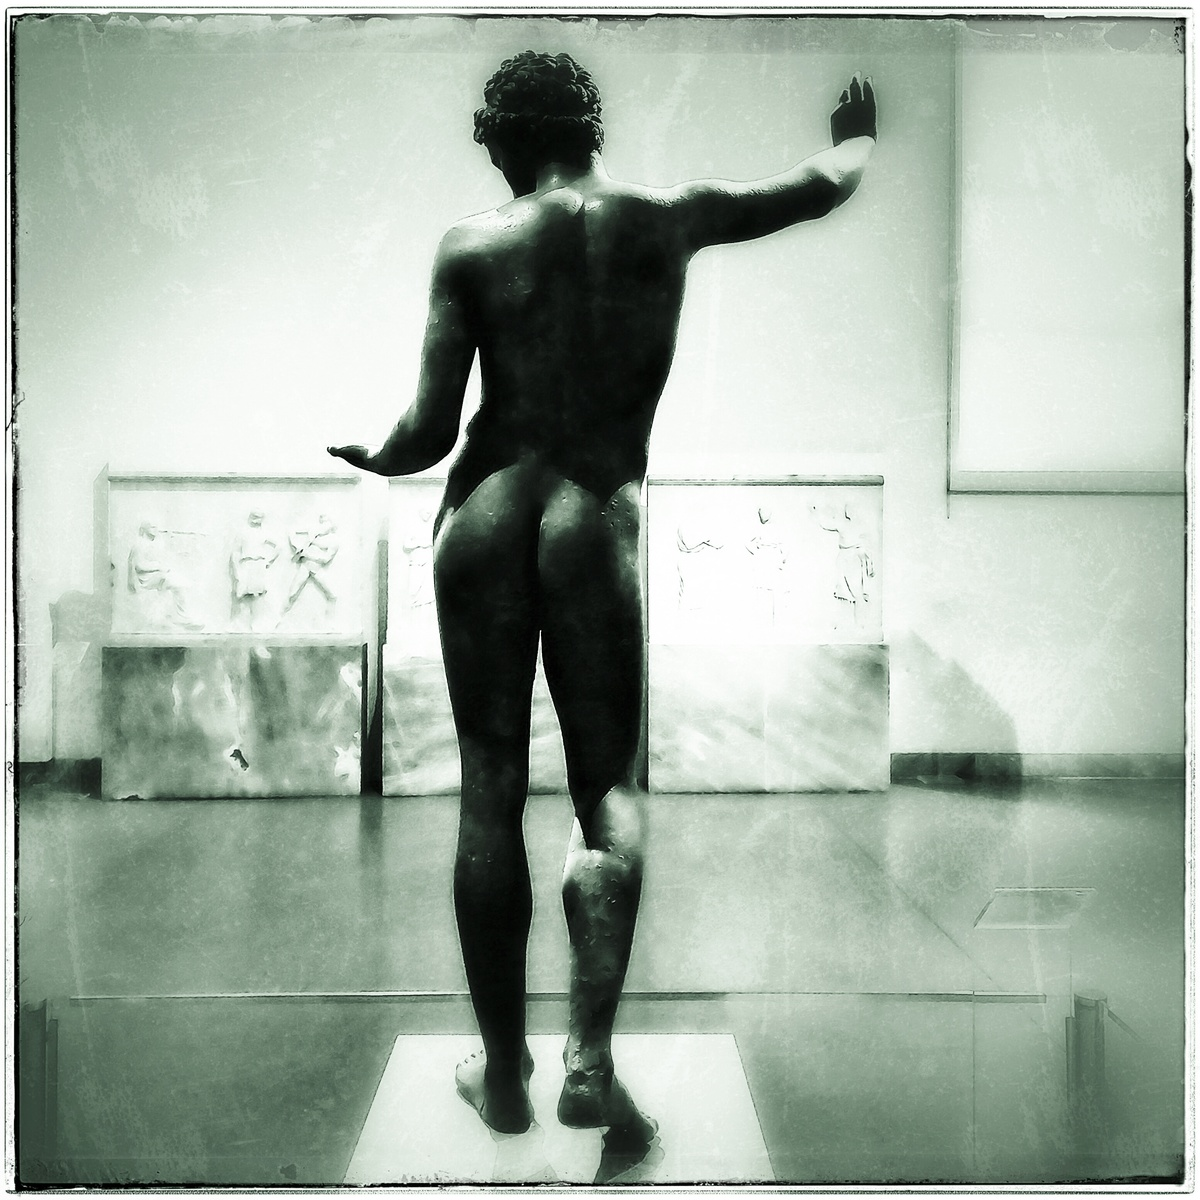
\includegraphics[width=0.8\linewidth]{thumb-lesson_VII.jpeg}
  %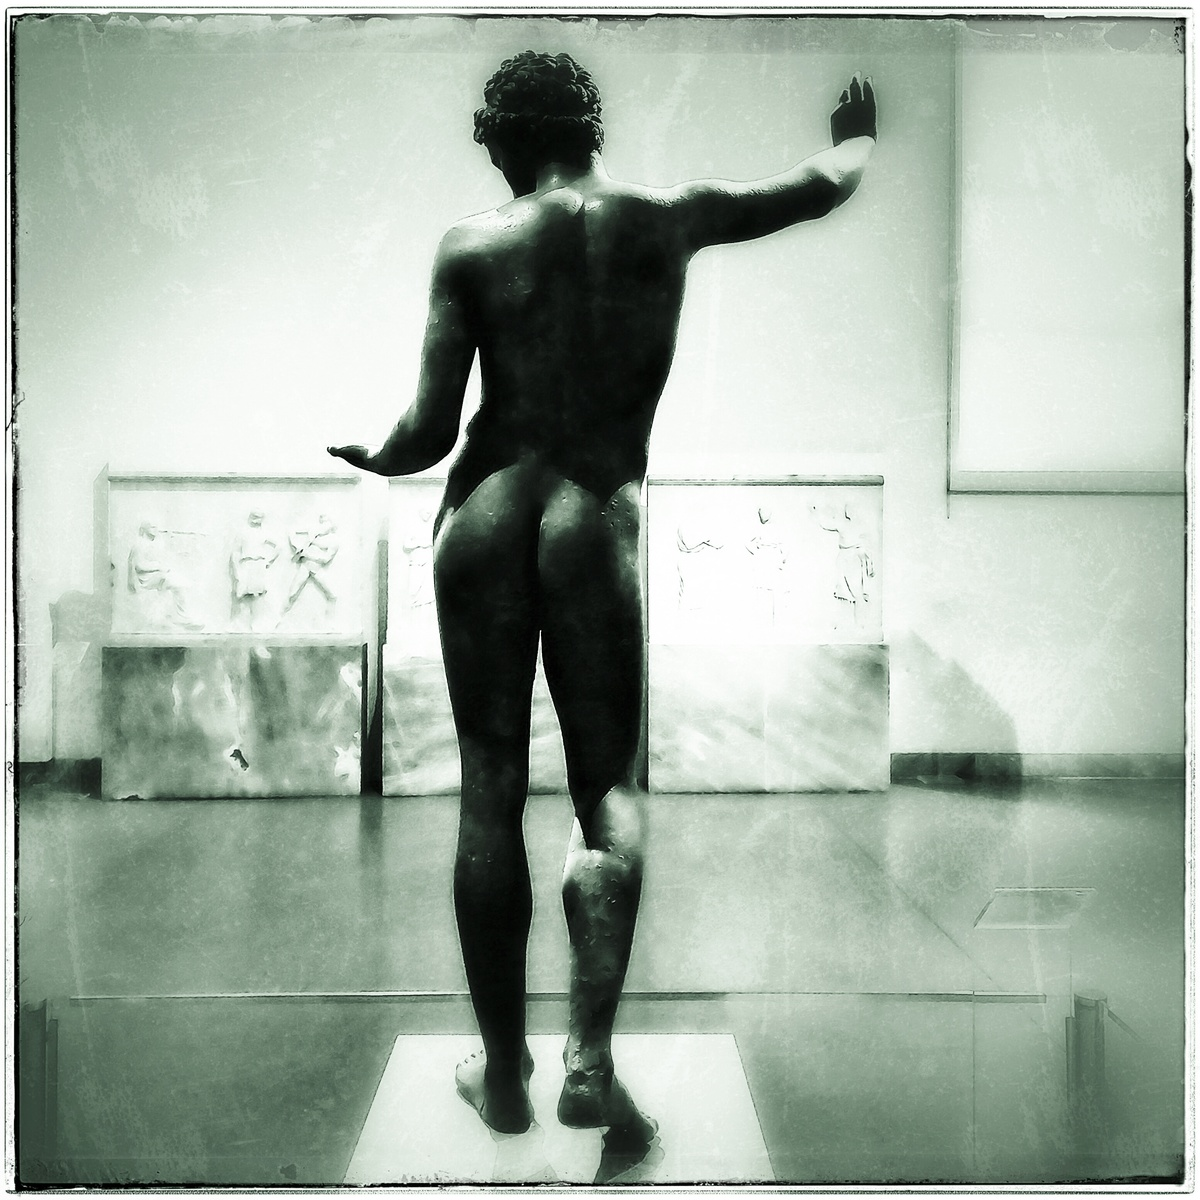
\includegraphics{thumb-lesson_VII.jpeg}
  \caption{Pavia: Almo Collegio Borromeo}
  \label{fig:textfig}
  %\zsavepos{pos:textfig}
  %\setfloatalignment{b}
\end{figure}

 

\nobibliography{latinBiblio}
\bibliographystyle{alpha}


\end{document}
